
\chapter{Les opérateurs dans le formalisme de Feynman} % III
% 25

L'idée centrale du formalisme de Feynman est d'associer une
amplitude de probabilité à chaque chemin, ou histoire, du système entre
un état initial et un état final donnés. La même idée permet de définir
de façon très simple l'opérateur {\it quantique} G qui correspond à une grandeur
{\it classique} g. (Nous réservons de façon systématique les minuscules aux
grandeurs classiques et les majuscules aux grandeurs quantiques.).

Après avoir défini et étudié les opérateurs dans le formalisme
de Feynman et établi le lien avec le formalisme habituel de la mécanique
quantique pour des cas de plus en plus compliqués (\S A, B, C), nous
appliquons les résultats de cette étude à un problème important, celui de la
théorie des perturbations dépendant du temps (\S D).

\section{Opérateurs relatifs à un instant donné t$_\mt{k}$}
\subsection{Définition de Feynman} % 1°)

Nous allons tout d'abord adopter pour l'amplitude de probabilité < x" t'' | x' t' > la notation plus commode

\[
\mt{<x''t''|x't'>} = \sum_\mt{H} \mt{N exp} \frac{\mt{i}}{\hbar} \mt{S}_\mt{H} =
\lim_{\,\epsilon \to \,0} \frac{1}{\mt{A}}
\int \frac{\mt{dx}_1}{\mt{A}}..\frac{\mt{dx}_{\mt{n-1}}}{\mt{A}}
\mt{exp} \frac{\mt{i}}{\hbar} \sum_\mt{i=0}^\mt{n-1}
\mt{S (x}_\mt{i}, \mt{x}_\mt{i+1})
\]
qui n'est autre qu'une forme condensée de la formule (2) au chapitre II, dans
laquelle $\sum_{H}$ représente la sommation sur tous les chemins, ou histoires 
possibles, telle qu'elle a été définie dans les postulats, S$_\mt{H}$ l'action 
pour le chemin H.
%26
\subsubsection{Opérateur position à l'instant t$_\mt{k}$, x(t$_\mt{k}$)}%a) 

\begin{center} 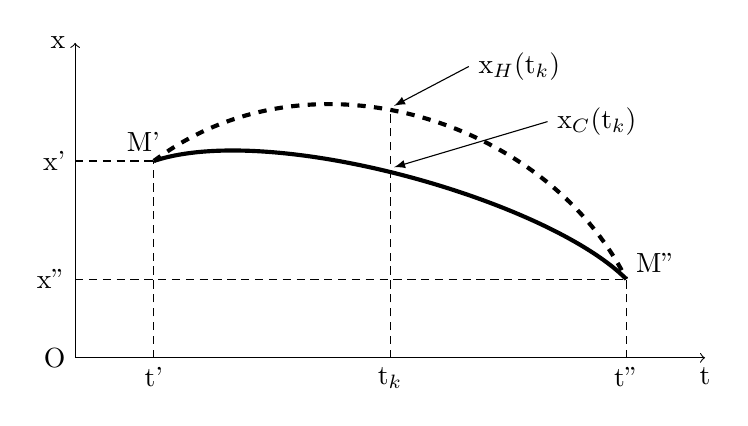
\begin{tikzpicture}
% axes
\draw [->] (0,0) --++ (8,0) node [below] {t};
\draw [->] (0,0) --++ (0,4) node [left] {x};
\node at (0,0) [left]{O};
% coordonnées et points
\draw [densely dashed] (0,2.5) node [left] {x'} --++ (1,0);
\draw [densely dashed] (1,0) node [below] {t'} --++ (0,2.5);
\node at (1.2,2.5) [above left]{M'};
\draw [densely dashed] (0,1) node [left] {x''} --++ (7,0);
\draw [densely dashed] (7,0) node [below] {t''} --++ (0,1);
\node at (7,1.2) [right]{M''};
%  milieu
\draw [densely dashed] (4,-0) node [below] {t$_\mt{k}$} -- (4,2.4) -- (4, 3.15);
\draw [<-, >=latex] (4.05, 2.42) -- (6, 3) node [right]{x$_\mt{C}$(t$_\mt{k}$)};
\draw [<-, >=latex] (4.05, 3.2) -- (5, 3.7) node [right]{x$_\mt{H}$(t$_\mt{k}$)};
% Chemins
\draw [line width=1.5pt] (1,2.5) .. controls (2.5,3) and (6,2) .. (7,1);
\draw [line width=1.5pt, dashed] (1,2.5) .. controls (3,4) and (6,3) .. (7,1);
\end{tikzpicture} \end{center}
Entre deux points M' et M'' de l'espace-temps, nous savons
qu'une {\it particule classique} suit un chemin {\it bien défini}, celui de l'action
{\it stationnaire} (en trait plein sur la figure). Sa position à l'instant t$_\mt{k}$,
x$_\mt{C}$(t$_\mt{k}$), est donc elle aussi bien {\it définie}.

En mécanique quantique, au contraire, la situation est totalement différente. L'amplitude de probabilité < x''t'' | x't' > est la somme
des amplitudes associées à {\it tous} les chemins ou histoires possibles reliant
M à M" et on peut donc dire que la particule est passée à l'instant t$_\mt{k}$, par
{\it toutes} les positions x$_\mt{H}$(t$_\mt{k}$), relatives à {\it toutes} les histoires H.

Il est alors naturel d'envisager la quantité
N$\sum_\mt{H} \mt{x}_\mt{H} (\mt{t}_\mt{k}) \mt{exp} \frac{\mt{i}}{\hbar} \mt{S}_\mt{H}$
obtenue en pondérant la valeur x$_\mt{H}$(t$_\mt{k}$) par l'amplitude de probabilité associée
au chemin correspondant, N exp$\frac{\mt{i}}{\hbar} \mt{S}_\mt{H}$ et en sommant sur toutes les histoires
possibles entre M' et M''.

{\it }Par définition, Feynman appelle la quantité précédente 1'{\it élément
de matrice entre les états} < x''t'' | et | x't' > {\it de l'opérateur} X(t$_\mt{k}$) {\it associé
à la grandeur physique, position à l'instant} t$_\mt{k}$, x(t$_\mt{k}$)
On adopte la notation :
\[
\tag{1}\subset \mt{x''t''} | \mt{X(t}_\mt{k}) | \mt{x't'}\supset =
\mt{N}\sum_\mt{H} \mt{x}_\mt{H} (\mt{t}_\mt{k}) \mt{exp} \frac{\mt{i}}{\hbar} \mt{S}_\mt{H}
=\lim_{\epsilon \to \,0} \frac{1}{\mt{A}}
\int \frac{\mt{dx}_1}{\mt{A}}..\frac{\mt{dx}_{\mt{n-1}}}{\mt{A}} \mt{x}_\mt{k}
\mt{exp} \frac{\mt{i}}{\hbar} \sum_\mt{i=0}^\mt{n-1}
\mt{S (x}_\mt{i}, \mt{x}_\mt{i+1})
\]
%27

{\bf Remarques}

$\alpha$) Pour marquer la différence entre les éléments de matrice au sens de
Feynman et les éléments de matrice au sens habituel de la mécanique
quantique, nous avons adopté la notation $\subset |\ | \supset$ différente de celle de
Dirac $< |\ | >$ . Nous constaterons que ces deux notations ne sont pas
toujours équivalentes.

$\beta$) Quelle est la limite de la quantité
$\frac{\subset \mt{x''t''} | \mt{X(t}_\mt{k}) | \mt{x't'}\supset}{\mt{<x''t''|x't'>}}$
lorsque  $\hbar \to 0$ (limite classique) ?

Il est clair d'après la relation (1) que les seules contributions à
$\subset \mt{x''t''} | \mt{X(t}_\mt{k}) | \mt{x't'}\supset$
qui ne se détruisent pas par interférence
sont celles qui correspondent au voisinage du chemin classique de l'action
stationnaire et qu'alors la quantité
$\frac{\subset \mt{x''t''} | \mt{X(t}_\mt{k}) | \mt{x't'}\supset}{\mt{<x''t''|x't'>}}$
qui est bien homogène à une longueur, tend vers x$_\mt{C}$(t$_\mt{k}$).

\subsubsection{Autres opérateurs} % b)
Les résultats précédents ont une généralisation immédiate :
Soit g(t) une grandeur physique que l'on peut définir à l'instant t$_\mt{k}$, pour
toute histoire H de la particule.  g$_\mt{C}$(t$_\mt{k}$) représente la grandeur relative
à la trajectoire classique et g$_\mt{H}$(t$_\mt{k}$) la grandeur relative à l'histoire H.

Par définition, on appelle élément de matrice au sens de
Feynman entre < x't' | et | x't' > de l'opérateur G(t$_\mt{k}$), correspondant à
la grandeur physique g, la quantité
\[
\subset \mt{x''t''} | \mt{G(t}_\mt{k}) | \mt{x't'}\supset =
\sum_\mt{H}\mt{N} \mt{g}_\mt{H} (\mt{t}_\mt{k}) \mt{exp} \frac{\mt{i}}{\hbar} \mt{S}_\mt{H}
\]
{\bf Remarque} : Comment peut-on définir la vitesse à l'instant t$_\mt{k}$ ?

\begin{center} 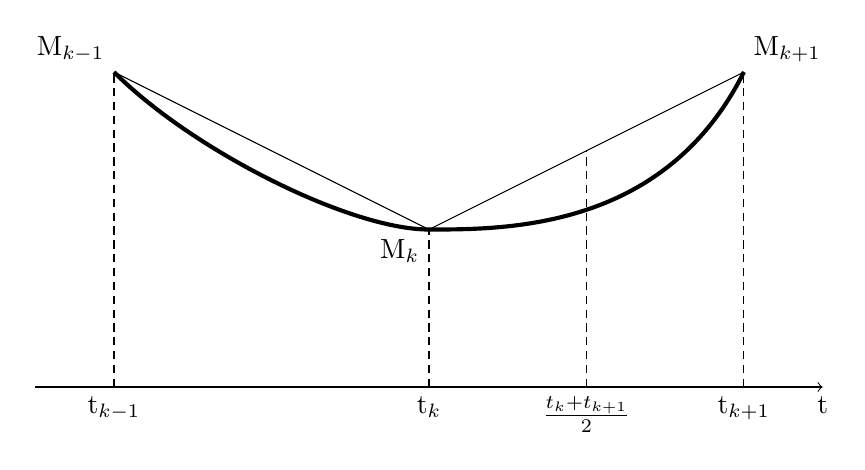
\begin{tikzpicture}
\coordinate (A) at (1,4) ;
\coordinate (B) at (5,2) ;
\coordinate (C) at (9,4) ;
% axe
\draw [->] (0,0) --++ (10,0) node [below] {t};
% ordonnées et points
\draw [densely dashed] (1,0) node [below] {t$_\mt{k-1}$} -- (A) node [above left]{M$_\mt{k-1}$};
\draw [densely dashed] (5,0) node [below] {t$_\mt{k}$} -- (B) node [below left]{M$_\mt{k}$};
\draw [densely dashed] (9,0) node [below] {t$_\mt{k+1}$} -- (C) node [above right]{M$_\mt{k+1}$};
\draw [densely dashed] (7,0) node [below] {$\frac{\mt{t}_\mt{k}+\mt{t}_\mt{k+1}}{2}$} -- (7,3);
% segments
\draw (A) -- (B) -- (C);
% Chemins
\draw [line width=1.5pt] (A) .. controls (2,3) and (4,2) .. (B);
\draw [line width=1.5pt] (B) .. controls (6,2) and (8,2) .. (C);
\end{tikzpicture} \end{center}
% 28

Rappelons que les chemins H sont en fait définis par une
suite de points M', ... M$_\mt{k-1}$, M$_\mt{k}$, M$_\mt{k+1}$, ... M", reliés les uns aux autres
par des chemins classiques infinitésimaux. Il résulte de cette définition
que la grandeur classique "vitesse au point t$_\mt{k}$" n'est pas définie, puisque
la dérivée $\dot{\mt{x}}$(t) est discontinue en ce point. On convient alors de définir
\[
\mt{v(t}_\mt{k}) =
\lim_{\epsilon \to \,0} \frac{\mt{x(t}_{\mt{k+1}}) - \mt{x(t}_\mt{k})}{\epsilon}
\]
De même, pour la grandeur physique "produit de la position par la vitesse
à l'instent t$_\mt{k}$", on prend, au lieu de x (t$_\mt{k}$) v (t$_\mt{k}$), qui n'est pas défini,
la quantité
\[
\lim_{\epsilon \to \,0} \frac{\mt{x(t}_\mt{k}) + \mt{x(t}_\mt{k+1})}{2}
\ \frac{\mt{x(t}_{\mt{k+1}}) - \mt{x(t}_\mt{k})}{\epsilon}
\]

Ces définitions reviennent à envisager les grandeurs physiques
corresrondantes à un {\it même} instant, par exemple
$\frac{\mt{t}_\mt{k} + \mt{t}_\mt{k+1}}{2}$, où elles sont
définies et à prendre pour chemin classique entre M$_\mt{k}$ et M$_\mt{k+1}$ une droite
d'espace-temps. Ces deux approximations sont justifiées par le fait qu'on
prend les limites des expressions précédentes pour $\epsilon \to \,0$.

(Nous savons (cf ch. II, note p. 22) qu'on peut approcher le chemin classique
M$_\mt{k}$ M$_\mt{k+1}$ par une droite, ce qui justifie la définition ci-dessus
de x(t$_\mt{k}$) v(t$_\mt{k}$) qui correspond à la limite pour $\epsilon \to \,0$
de x($\frac{\mt{t}_\mt{k} + \mt{t}_\mt{k+1}}{2}$)v($\frac{\mt{t}_\mt{k} + \mt{t}_\mt{k+1}}{2}$).
On pourrait envisager d'adopter la définition plus simple
x(t$_\mt{k}$)v(t$_\mt{k}) =
\lim_{\epsilon \to \,0}$ x(t$_\mt{k}$) $\epsilon^{-1}[\mt{x(t}_\mt{k+1}) - \mt{x(t}_\mt{k})]$.
On commet alors sur x(t) une erreur qui peut être en $\epsilon^{1/2}$ et, comme v
peut croître en $\epsilon^{-1/2}$ (cf note p. 22) une erreur sur x(t$_\mt{k}$)v(t$_\mt{k}$) qui peut
rester finie lorsque $\epsilon \to \,0$. Il est donc bien indispensable d'envisager les
grandeurs physiques x(t) et v(t) à un {\it même} instant.)

\subsection{Lien avec le formalisme habituel de la mécanique quantique}% 2°)

\subsubsection{Point de vue de Heisenberg}% a)
L'élément de matrice $\subset \mt{x''t''} | \mt{X(t}_\mt{k}) | \mt{x't'}\supset$ peut s'écrire
en divisant en trois parties l'intégration sur les chemins :
\[
\tag{2}\subset \mt{x''t''} | \mt{X(t}_\mt{k}) | \mt{x't'}\supset =
\lim_{\epsilon \to \,0} \int \mt{x}_\mt{k}\mt{dx}_\mt{k} \left[\frac{1}{\mt{A}}
\int...\int \frac{\mt{dx}_1}{\mt{A}}..\frac{\mt{dx}_\mt{k-1}}{\mt{A}}
\mt{exp} \frac{\mt{i}}{\hbar} \sum_\mt{i=0}^\mt{k-1}
\mt{S (x}_\mt{i}, \mt{x}_\mt{i+1})\right]
\]
\[
\times \left[\frac{1}{\mt{A}}
\int...\int \frac{\mt{dx}_\mt{k+1}}{\mt{A}}..\frac{\mt{dx}_\mt{n-1}}{\mt{A}}
\mt{exp} \frac{\mt{i}}{\hbar} \sum_\mt{i=k}^\mt{n-1}
\mt{S (x}_\mt{i}, \mt{x}_\mt{i+1})\right]
\]
%29
Or $\lim_{\epsilon \to \,0} \frac{1}{\mt{A}}
\int...\int \frac{\mt{dx}_1}{\mt{A}}..\frac{\mt{dx}_\mt{k-1}}{\mt{A}}
\mt{exp} \frac{\mt{i}}{\hbar} \sum_\mt{i=0}^\mt{k-1}
\mt{S (x}_\mt{i}, \mt{x}_\mt{i+1}) = $ < x$_\mt{k}$t$_\mt{k}$ | x't' >

(par définition : cf chapitre II, formule 2)

De même $\lim_{\epsilon \to \,0} \frac{1}{\mt{A}}
\int...\int \frac{\mt{dx}_{k+1}}{\mt{A}}..\frac{\mt{dx}_\mt{n-1}}{\mt{A}}
\mt{exp} \frac{\mt{i}}{\hbar} \sum_\mt{i=k}^\mt{n-1}
\mt{S (x}_\mt{i}, \mt{x}_\mt{i+1}) = $ < x''t'' | x$_\mt{k}$t$_\mt{k}$ >

(2) devient alors
\begin{center}
$\subset \mt{x''t''} | \mt{X(t}_\mt{k}) | \mt{x't'}\supset = \int \mt{dx}_\mt{k}
 < \mt{x''t''} | \mt{x}_\mt{k}\mt{t}_\mt{k} >
 \mt{x}_\mt{k}
 < \mt{x}_\mt{k}\mt{t}_\mt{k} | \mt{x't'} > $
\end{center}
Or on a x$_\mt{k} \delta$(x'$_\mt{k} -$ x$_\mt{k}$) =
< x$_\mt{k}$t$_\mt{k}$ | X(t$_\mt{k}$)| x'$_\mt{k}$t$_\mt{k}$ >
(les éléments de matrice sont ici pris au sens habituel de Heisenberg)

Finalement, on peut donc écrire
\[
\tag{3}\subset \mt{x''t''} | \mt{X(t}_\mt{k}) | \mt{x't'}\supset\ =
\int\int \mt{dx}_\mt{k} \mt{dx'}_\mt{k}
 < \mt{x''t''} | \mt{x}_\mt{k}\mt{t}_\mt{k} >
 < \mt{x}_\mt{k}\mt{t}_\mt{k} | \mt{X(t}_\mt{k})| \mt{x'}_\mt{k}\mt{t}_\mt{k} >
 < \mt{x'}_\mt{k}\mt{t}_\mt{k} | \mt{x't'} >
\]
\begin{center}
$ = < \mt{x''t''} | \mt{X(t}_\mt{k})| \mt{x't'} >$
\end{center}

Il y a donc accord entre la définition de Feynman et la définition habituelle
des éléments de matrice (éans le point de vue de Heisenberg).
\subsubsection{Point de vue de Schrödinger}% b)

Nous appellerons \underline{X} l'opérateur X(t) dans le point de vue de
Schrödinger.

On calcule alors $\subset \mt{x''t''} | \mt{X(t}_\mt{k}) | \mt{x't'}\supset$ à partir de la
formule (3) ci-dessus en remarquant que
\begin{center}
$< \mt{x}_\mt{k}\mt{t}_\mt{k} | \mt{X(t}_\mt{k})| \mt{x'}_\mt{k}\mt{t}_\mt{k} >
= < \mt{x}_\mt{k} | \underline{\mt{X}} | \mt{x'}_\mt{k} >
=\mt{x}_\mt{k}\delta(\mt{x}_\mt{k}-\mt{x'}_\mt{k})$

$< \mt{x''t''} | \mt{x}_\mt{k}\mt{t}_\mt{k} > =
< \mt{x''} | \mt{U(t'',t}_\mt{k})| \mt{x}_\mt{k} >$

$< \mt{x'}_\mt{k}\mt{t}_\mt{k} | \mt{x't'} > =
< \mt{x'}_\mt{k} | \mt{U(t}_\mt{k},\mt{t')}| \mt{x'} >$

(cf chapitre II)
\end{center}

%30
(3) s'écrit alors
\[
\tag{4}\subset \mt{x''t''} | \mt{X(t}_\mt{k}) | \mt{x't'}\supset\ =
\int\int \mt{dx}_\mt{k} \mt{dx'}_\mt{k}
 < \mt{x''} | \mt{U(t'',t}_\mt{k})| \mt{x}_\mt{k} >
 < \mt{x}_\mt{k} | \underline{\mt{X}} | \mt{x'}_\mt{k} >
 < \mt{x'}_\mt{k} | \mt{U(t}_\mt{k},\mt{t')}| \mt{x'} >
\]\[
=< \mt{x''} | \mt{U(t'',t}_\mt{k}) \underline{\mt{X}} \mt{U(t}_\mt{k},\mt{t')}| \mt{x'} >
\]
Remarque :

\begin{minipage}[c]{.15\linewidth}
Posons
\end{minipage}
%\hfill
\begin{minipage}[c]{.35\linewidth}
$|\chi>=\mt{U}^\dagger\mt{(t'',t}_\mt{k})| \mt{x''} >$

$|\psi> = \mt{U(t}_\mt{k},\mt{t')}| \mt{x'} >$
\end{minipage}
\hfill

$|\psi>$ représente l'état à l'instant t$_\mt{k}$ de la particule qui a été localisée
en x' à l'instant t' < t$_\mt{k}$.
$|\chi>$ représente l'état à l'instant t$_\mt{k}$ de la particule qui sera localisée en
x'' à l'instant t'' > t$_\mt{k}$.

On a alors d'après la relation (4) :
\[
\subset \mt{x''t''} | \mt{X(t}_\mt{k}) | \mt{x't'}\supset\ =
<\chi| \underline{\mt{X}} |\psi>
\]
On voit ainsi que l'élément de matrice au sens de Feynman n'est
autre que l'élément de matrice ordinaire à l'instant t$_\mt{k}$ de l'opérateur position \underline{X}, entre l'état physique qui a évolué à partir de la particule localisée
en x' à l'instant t' < t$_\mt{k}$ et l'état qui évoluera à l'instant t'' > t$_\mt{k}$ vers
la particule localisée au point x''. L'élément de matrice au sens de Feynman
ne peut donc en aucun cas être considéré comme une valeur moyenne, résultat
d'une mesure de la grandeur x(t$_\mt{k}$) puisqu'il correspond à un élément de
matrice pris entre {\it deux états différents} $<\chi|$ et $|\psi>$.

\section{Produits de deux orérateurs relatifs à des instants différents t$_\mt{k}$, t$_\mt{l}$}% B. 
\subsection{Définition de Feynman}% 1°) 

De même que nous avons, au paragraphe .1, défini des opérateurs
relatifs à un instant donné t$_\mt{k}$, nous allons étendre cette définition à deux
instants différents t$_\mt{l}$ et t$_\mt{k}$ en posant par exemple t$_\mt{l}$ > t$_\mt{k}$.

%-31
Prenons d'abord pour exemple la grandeur physique x(t$_\mt{k}$) x(t$_\mt{l}$)
produit de la position de la particule à deux instants différents.

Pour une particule classique décrivant M' M'', nous savons que
cette grandeur prend la valeur bien définie  x$_\mt{C}$(t$_\mt{k}$) x$_\mt{C}$(t$_\mt{l}$).

A chaque histoire H contribuant à l'amplitude de probabilité
quantique < x''t'' | x't' > on associe le nombre x$_\mt{H}$(t$_\mt{k}$) x$_\mt{H}$(t$_\mt{l}$).

On définit alors l'élément de matrice au sens de Feynman entre
les états < x''t'' | et | x't' > du produit d'opérateurs X(t$_\mt{k}$) X(t$_\mt{l}$) aux
deux instants t$_\mt{k}$ et t$_\mt{l}$ par la relation
\[
\tag{5}\subset \mt{x''t''} | \mt{X(t}_\mt{k}) \mt{ X(t}_\mt{l}) | \mt{x't'}\supset\ =
\sum_H \mt{N x}_\mt{H}(\mt{t}_\mt{k}) \mt{ x}_\mt{H}(\mt{t}_\mt{l})
\mt{ exp}\frac{\mt{i}}{\hbar}\mt{S}_\mt{H}
\]
Remarque :

À la limite classique où $\hbar \to 0$, on montre, comme au paragraphe 1 :
$$ \lim_{\hbar \to 0} \frac{\subset \mt{x''t''} | \mt{X(t}_\mt{k}) \mt{ X(t}_\mt{l}) | \mt{x't'}\supset}
{< \mt{x''t''} | \mt{x't'}>} = \mt{ x}_\mt{C}(\mt{t}_\mt{k}) \mt{ x}_\mt{C}(\mt{t}_\mt{l})$$
Les définitions précédentes se généralisent immédiatement :
Soient f(t$_\mt{k}$) et g(t$_\mt{l}$) deux grandeurs rhysiques aux instants t$_\mt{k}$ et t$_\mt{l}$,
f$_\mt{H}$(t$_\mt{k}$) et g$_\mt{H}$(t$_\mt{l}$) les valeurs de ces grandeurs pour une histoire H; alors
la quantité :
\[
\tag{6}\subset \mt{x''t''} | \mt{F(t}_\mt{k}) \mt{ G(t}_\mt{l}) | \mt{x't'}\supset\ =
\sum_H \mt{N f}_\mt{H}(\mt{t}_\mt{k}) \mt{ g}_\mt{H}(\mt{t}_\mt{l})
\mt{ exp}\frac{\mt{i}}{\hbar}\mt{S}_\mt{H}
\]
représente l'élément de matrice au sens de Feynman entre les états < x't' |
et | x''t'' > du produit des opérateurs $\mt{F(t}_\mt{k}) \mt{ G(t}_\mt{l})$ aux deux instants t$_\mt{k}$
et t$_\mt{l}$.

{\bf Remarque importante :} D'après les formules (5) et (6), il résulte de la commutation des nombres
x$_\mt{H}$(t$_\mt{k}$) x$_\mt{H}$(t$_\mt{l}$), que les opérateurs au sens de Feynman à deux instants
différents commutent :
\[
\subset \mt{x''t''} | \mt{X(t}_\mt{k}) \mt{ X(t}_\mt{l}) | \mt{x't'}\supset\ =
\subset \mt{x''t''} | \mt{X(t}_\mt{l}) \mt{ X(t}_\mt{k}) | \mt{x't'}\supset\
\]
\[
\subset \mt{x''t''} | \mt{F(t}_\mt{k}) \mt{ G(t}_\mt{l}) | \mt{x't'}\supset\ =
\subset \mt{x''t''} | \mt{G(t}_\mt{l}) \mt{ F(t}_\mt{k}) | \mt{x't'}\supset\
\]
L'ordre dans lequel sont rangés les instants t$_\mt{k}$ et t$_\mt{l}$ n'importe pas.
%32

\subsection{Lien avec le formalisme habituel}% 2°)
\subsubsection{Point de vue de Heisenberg}% a)

La formule (5) s'écrit :
\[
\tag{7}\subset \mt{x''t''} | \mt{X(t}_\mt{k}) \mt{ X(t}_\mt{l}) | \mt{x't'}\supset\ =
\lim_{\epsilon \to \,0} \frac{1}{\mt{A}}
\int...\int \frac{\mt{dx}_1}{\mt{A}}..\frac{\mt{dx}_\mt{n-1}}{\mt{A}}
\mt{x}_\mt{k}\mt{x}_\mt{l}
\mt{exp} \frac{\mt{i}}{\hbar} \sum_\mt{i=0}^\mt{n-1}
\mt{S (x}_\mt{i}, \mt{x}_\mt{i+1})
\]
Par un raisonnement analogue à celui déjà fait au \S 1, (7) devient
\[
\subset \mt{x''t''} | \mt{X(t}_\mt{k}) \mt{ X(t}_\mt{l}) | \mt{x't'}\supset\ =
\lim_{\epsilon \to \,0}\int\int\mt{x}_\mt{k}\mt{x}_\mt{l}\mt{dx}_\mt{k}\mt{dx}_\mt{l}
\left[\frac{1}{\mt{A}}\int...\int\frac{\mt{dx}_1}{\mt{A}}..\frac{\mt{dx}_\mt{k-1}}{\mt{A}}
\mt{exp} \frac{\mt{i}}{\hbar} \sum_\mt{i=0}^\mt{k-1}\mt{S (x}_\mt{i}, \mt{x}_\mt{i+1})\right.
\]
\[
\left.\times\frac{1}{\mt{A}}\int...\int\frac{\mt{dx}_\mt{k+1}}{\mt{A}}..\frac{\mt{dx}_\mt{l-1}}{\mt{A}}
\mt{exp} \frac{\mt{i}}{\hbar} \sum_\mt{i=k}^\mt{l-1}\mt{S (x}_\mt{i}, \mt{x}_\mt{i+1})
\times\frac{1}{\mt{A}}\int...\int\frac{\mt{dx}_\mt{l+1}}{\mt{A}}..\frac{\mt{dx}_\mt{n-1}}{\mt{A}}
\mt{exp} \frac{\mt{i}}{\hbar} \sum_\mt{i=l}^\mt{n-1}\mt{S (x}_\mt{i}, \mt{x}_\mt{i+1})\right]
\]
\[
= \int\int \mt{dx}_\mt{k} \mt{dx}_\mt{l}
< \mt{x''t''} | \mt{x}_\mt{l}\mt{t}_\mt{l} > \mt{x}_\mt{l}
< \mt{x}_\mt{l}\mt{t}_\mt{l} | \mt{x}_\mt{k}\mt{t}_\mt{k} >
\mt{x}_\mt{k}< \mt{x}_\mt{k}\mt{t}_\mt{k} | \mt{x't'} >
\]
\[
= \int\int\int\int \mt{dx}_\mt{k} \mt{dx'}_\mt{k} \mt{dx}_\mt{l} \mt{dx'}_\mt{l}
 < \mt{x''t''} | \mt{x}_\mt{l}\mt{t}_\mt{l} >
 < \mt{x}_\mt{l}\mt{t}_\mt{l} | \mt{X(t}_\mt{l})| \mt{x'}_\mt{l}\mt{t}_\mt{l} >
 < \mt{x}_\mt{l}\mt{t}_\mt{l} | \mt{x}_\mt{k}\mt{t}_\mt{k} >
\]
\[
 < \mt{x}_\mt{k}\mt{t}_\mt{k} | \mt{X(t}_\mt{k})| \mt{x'}_\mt{k}\mt{t}_\mt{k} >
 < \mt{x'}_\mt{k}\mt{t}_\mt{k} | \mt{x't'} >
\]
\[
= < \mt{x''t''} | \mt{ X(t}_\mt{l}) \mt{X(t}_\mt{k})| \mt{x't'} >
\]
On a donc finalement
\[
\subset \mt{x''t''} | \mt{X(t}_\mt{k}) \mt{ X(t}_\mt{l}) | \mt{x't'}\supset\ =
< \mt{x''t''} | \mt{ X(t}_\mt{l}) \mt{X(t}_\mt{k}) | \mt{x't'} >
\ \ \ \ \ \ \mt{avec } \mt{t}_\mt{k} < \mt{t}_\mt{l}
\]
{\bf Remarque très importante :}
I1 résulte de la démonstration que nous venons de faire que dans l'élément
de matrice du point de vue de Heisenberg, les temps sont rangés dans l'ordre
croissant de la droite vers la gauche :
\[
\mt{t'} < \mt{t}_\mt{k} < \mt{t}_\mt{l} < \mt{t''}.
\]
%-33
Les opérateurs X(t$_\mt{l}$) et X(t$_\mt{k}$) relatifs à deux instants t$_\mt{k}$ et t$_\mt{l}$ différents
ne commutent pas (nar exemple, X(t) ne peut commuter avec X(t + $\epsilon$), car
on ne peut mesurer simultanément position et vitesse d'une particule)
\begin{center}
X (t$_\mt{l}$) X (t$_\mt{k}$) $\neq$ X (t$_\mt{k}$) X (t$_\mt{l}$)
\end{center}
Introduisons l'opérateur d'ordre P qui, au produit X (t$_\mt{l}$) X (t$_\mt{k}$), associe
X (t$_\mt{l}$) X (t$_\mt{k}$) si t$_\mt{k}$ < t$_\mt{l}$
et X (t$_\mt{k}$) X (t$_\mt{l}$) t$_\mt{k}$ > t$_\mt{l}$:

\[
\mt{P}[\mt{ X(t}_\mt{l}) \mt{X(t}_\mt{k})] = 
\left\{
  \begin{array}{rcr}
    \mt{X(t}_\mt{k}) \mt{ X(t}_\mt{l}) & \mt{si} & \mt{t}_\mt{k} < \mt{t}_\mt{l} \\
    \mt{X(t}_\mt{l}) \mt{ X(t}_\mt{k}) & \mt{si} & \mt{t}_\mt{k} > \mt{t}_\mt{l} \\
  \end{array}
\right.\]
Alors on a la relation fondamentale :

\[
\tag{8}\subset \mt{x''t''} | \mt{X(t}_\mt{k}) \mt{ X(t}_\mt{l}) | \mt{x't'}\supset\ =
\subset \mt{x''t''} | \mt{ X(t}_\mt{l}) \mt{X(t}_\mt{k}) | \mt{x't'}\supset\
\]
\[
 = < \mt{x''t''} | \mt{P}[\mt{ X(t}_\mt{l}) \mt{X(t}_\mt{k})] | \mt{x't'} >
\]
{\bf En résumé} : alors que les opérateurs associés à des temps différents commutent au sens de Feynman, il n'en est pas de même au point de vue de Heisenberg.
L'ordre qu'il faut alors adopter est celui des temps croissants de la droite
vers la gauche.
\subsubsection{Point de vue de Schrödinger}% b)
On déduit immédiatement du point de vue de Heisenberg :

\[
\subset \mt{x''t''} | \mt{X(t}_\mt{k}) \mt{ X(t}_\mt{l}) | \mt{x't'}\supset\ =
< \mt{x''t''} | \mt{ X(t}_\mt{l}) \mt{X(t}_\mt{k}) | \mt{x't'} >
\]
De façon plus générale, si nous avons affaire à des grandeurs physiques

relatives à des instants ty tys ve th différents, nous introduisons

,
l'opérateur d'ordre P aui ronge les temps dans l'ordre croissant de la
droite vers la pauche et nous avons

%34

Remarques :
a) Nous comprenons maintenant la raison pour laquelle nous avons adopté,
pour désigner les éléments de matrice au sens de Feynman,une notation différente de celle de Heisenberg. La relation (10) nous montre en effet que
les deux notions ne sont pas identiques et qu'il faut, pour passer de l'une
à l'autre, ranger de façon convenable les opérateurs.
b) Que devient maintenant, dans le formalisme de Heisenberg, l'opérateur
associé à la prandeur physique  ?

Nous avons vu au paragraphe À qu'il faut, pour que cette

quantité soit définie, la remplacer par

Il lui correspond,dans le formalisme de Heisenberg, l'opérateur


Si l'on adopte donc la définition de Feynman pour les opérateurs
associés à une grandeur physique, on obtient très naturellement la règle de
symétrisation : l'opérateur quantique correspondant à un produit de grandeurs
physiques et le produit syrétrisé, Ce produit symétrisé est différent du

produit ordinaire si les opérateurs ne commutent pas.

\subsection{Cas général} % C.

Nous avons défini jusqu'à présent des opérateurs correspondant à

un ou plusieurs instants en nombre fini. Mous avons pu le faire, à la condition
de pouvoir associer à chaque histoire H de la particule définie par la
%35
suite () une grandeur classique 
Considérons maintenant que  ne dépend plus seulement d'une
suite finie de positions  mais, globalement, de tout le chemin

Nous définissons ainsi comme grandeur physique une fonctionnelle du
chemin  qui dépend de toute l'histoire H,

Dans les paragraphes À et B, nous avons envisagé des fonctionnelles particulièrement simples. Par exemnle :

Nous pouvons maintenant envisager des fonctionnelles beaucoup
plus générales. Par exemple :

Cette dernière fonctionnelle représente simplement l'action
pour l'histoire H. Comme nous l'avons déjà fait en À et B, nous définissons
l'élément de matrice au sens de Feynman entre les états  et 

de l'opérateur fonctionnel  correspondant à la grandeur classique
par la relation
par exemple on définit l'élément de matrice de l'opérateur action quantique

%-36
En résumé : le formalisme de Feynman nous a permis de définir les opérateurs à
quantiques, non plus par leur action sur un vecteur d'état  au système
envisagé à un instant donné t, mais plutôt par leurs éléments de matrice
entre deux états à des instants différents, ce qui les associe étroitement
à l'évolution du système entre t' et t''.

Ceci nous a permis de retrouver tout d'abord les opérateurs de
la mécanique quantique habituelle, en précisent de facon plus naturelle la
correspondance entre mécanique classique et quantique et en justifiant la
rèrle de symétrisation. Enfin, nous pouvons définir (formule 12) une classe
d'opérateurs beaucoup plus vaste, agissant sur tout un intervalle d'espacetemps, celle des onérateurs fonctionnels.

Pemarque imrortante : 
Tant que la grandeur classique  ne dépendait que d'une suite finie
d'instants  il a été possible de trouver l'équivalent de l'élément
de matrice de Feynman dans le point de vue de Heisenberg (formule 10). Dans
le cas où  est la fonctionnelle la plus rénérale du chemin H, la
formule (10) peut se rénéraliser formellement :

La formule (1) sipnifie que s'il est possible, d'une façon ou d'une autre,
de développer la fonctionnelle F en une série de produits dépendant d'une
suite d'instants  alors il faudra, pour passer au point de vue
de Heisenberg, ranger dans chacun des termes de la série les temps croissants
de la droite vers la rauche. Nous préciserons cette notion de façon naturelle

au paragraphe D,

\section{Application : Théorie des perturbations dépendant du temps} % D

Le formalisme de Feynman est particulièrement bien adapté à
l'étude des variations apportées à l'amplitude de probabilité < x''t'' | x't' >
par une perturbation du hamiltonien ou du larrangien du système. Nous allons

voir que l'on peut ainsi retrouver de façon très simple les résultats de la

théorie des perturbations dépendent du temps.

 % 37-

\subsection{}
1°) Position du problème

Considérons une particule dans un potentiel w (x, t).

Son lagrangien L s'écrit

et l'action S associée à une histoire H :

L'amplitude de probabilité relative au lagrangien L, que nous écrirons

ce qui s'écrit dans le point de vue de Schrôdinrer

U (t'', t') étant l'opérateur d'évolution de la particule dans le potentiel

On change maintenant le potentiel qui devient .
Le lagrangien L s'écrit alors :

l'action associée à une histoire H devient

Enfin l'amplitude de probabilité relative au système perturbé, < x''t'' | x't' >.

s'écrit

Le problème que l'on se pose est, connaissant l'amplitude de

et la perturbation w (x,t), de déterminer < x''t''fx't' >, où

ce qui revient au même, dans un point de vue plus familier, connaissant

et w (x,t), déterminer U,

% 38
Pour l'instant, nous ne faisons aucune hypothèse sur la
grandeur de la perturbation w(x,t).

Un cas particulier important est celui où ve (x,t) = 0.
Le système non perturbé est alors celui d'une particule libre dont on sait

déterminer exactement le propagateur < x''t'' | x't' > (cf chapitre II).

Le problème revient alors à déterminer, à partir de l'opérateur d'évolution

de la particule libre, celui de la particule se déplaçant dans un potentiel
quelconque dépendant du temps w (x,t).

\subsection{}
2°) Expression de < x''t'' | x't! >s

De (16), (17), (18) on déduit immédiatement

ce qui n'est autre que l'élément de matrice au sens de Feynman

 étant l'opérateur quantique associé à w et l'indice 5 étant là
rour rappeler que l'élément de matrice est relatif au système non perturbé.

Nous pouvons donner de l'expression précédente une interprétation physique imagée très simple :

La perturbation w multiplie la contribution de chaque chemin H à l'amplitude

de probabilité par un facteur de déphasage exp dt, La
modification globale de l'amplitude de probabilité s'obtient en sommant
tous ces déphasages sur les chemins. On peut dire, par analogie avec l'optique,
que la perturbation modifie "l'indice de réfraction" dans l'espace-temps et
que le calcul de perturbation se ramène à un calcul de variation d'indice.

% 39
Afin d'alléger les notations, posons :

W (t) dépend du temps explicitement et implicitement [par l'intermédiaire
de X t] . L'opérateur correspondant dans le point de vue de Schrôdinrer
n'a plus qu'une dépendance explicite dans le temps. Nous l'écrirons w (t).
Avec nos nouvelles notations, (19) s'écrit :

L'opérateur d'ordre P a été défini dans le paragraphe C. Nous ne pourrons lui
donner une signification précise qu'en développant l'exnronentielle en série,
L'indice O de la formule (21) rappelle que les états | x't' > et | x''t'' >
sont les états propres des opérateurs de Heisenberg X(t') et X(t'') de la

particule non perturbée.

\subsection{}
3°) Développerent en série de la perturbation ;


Développons en série :

Reportons ce développement dans la formule (20) : on obtient
%

Pour passer au point de vue de Heisenberg, nous devons faire
agir sur chaque terme de la série (22) l'opérateur d'ordre P.

(23) conduit alors à :

L'opérateur P va ranger, dans chaque intégrale les opérateurs W qui ne commutent pas dans le point de vue de Heisenberg par ordre de temps croissants
de la droite vers la gauche.

On montre la relation générale :

I1 existe n! façons de ranger les n variables dans un ordre
donné. Le région d'intégration de l'espace
 est constituée par la réunion des n! régions correspondant à

chacun de ces arrangements. L'intégrale I =
est la somme de n! intégrales prises sur chacune de ces régions, A chacune de
ces intégrales, l'onérateur d'ordre P, aui range les opérateurs par ordre de
temps croissants de la droite vers la gauche, fait correspondre par définition

la même intégrale



On a donc  ce qui n'est autre que la relation (25)

Les factorielles de la relation (24) ont disparu.
Passons maintenant au point de vue de Schrödinger :
(26) devient

ce qui nous donne le développerient de U en puissance de la perturbation :

%

Nous retrouvons ainsi le développement classique à tous les
ordres de la théorie des perturbations dépendant du temps (cf Messiah, tome II,
p. 620).
Remarque :
Le formalisme de FeYnman nous a permis d'obtenir, sans aucun calcul, une
forme symbolique et intégrée de ce développement à tous les ordres (formule 21)
grâce à l'introduction de l'opérateur d'ordre P,
En mécanique quantique habituelle, on procède de façon inverse.
On étebiit d'abord le développement (28) dans lequel les temps 
sont ordonnés. On s'affranchit ensuite de cet ordre en faisant apparaître artificiellement les factorielles qui conduisent à la relation (2h) et à la
forme symbolique (21).
Les calculs sont ainsi plus longs et plus compliqués que dans
le formalisme de Feynman dans lequel les opérateurs corresrondant à des temps
différents commutent,. Ce formalisme présente en outre le grand avantage de
donner une sisnification physique simple (en terme de modification de

l'indice de réfraction dans l'espace-temps) à la théorie des perturbations

dépendant du temps.

